\documentclass[11pt,a4paper]{article}
\usepackage[T1]{fontenc}
\usepackage{lmodern}
\usepackage[margin=2.5cm]{geometry}
\usepackage{amsmath,amssymb}
\usepackage{booktabs}
\usepackage{enumitem}
\usepackage{microtype}
\usepackage{placeins}
\usepackage{tikz}
\usetikzlibrary{arrows.meta}
\usepackage[hidelinks]{hyperref}

\newcommand{\code}[1]{\texttt{\detokenize{#1}}}
\newcommand{\gov}{\mathrm{gov}}
\newcommand{\GDP}{\mathit{GDP}}
\setlist{itemsep=2pt,topsep=4pt}
\setlength{\belowcaptionskip}{6pt}

\title{The public sector in GREU\\ Public industries, product flows, and the government budget}
\author{}
\date{23 November 2026}

\begin{document}
\maketitle

\section{Summary}

This note describes the public sector in the Julia version of GREU.
It shows the product flows into and out of the public industries.
It then explains how the model goes from the public industries to the government sector and its budget.

The numbers are from the baseline in \code{Output/baseline.parquet}.
They are for Denmark in 2019, the calibration year, in EUR million.

\begin{itemize}
\item The model has 63 industries, 63 products, and five sectors. An industry makes products. A sector owns production and has a budget. The model has no set of public industries, and no equation is special for them.
\item This note uses the name \emph{public industries} for four industries: public administration (O), education (P), health (Q86), and social work (Q87--88). They make 15 per cent of all output and employ 32 per cent of all persons.
\item Wages are 60 per cent of their output value, intermediate inputs are 31 per cent, and gross operating surplus is 9 per cent.
\item Government consumption takes 80 per cent of their output, households take 10 per cent, industries take 7 per cent, and exports and investment take 3 per cent.
\item One matrix of shares links industries to sectors. The government sector gets a share of the output, the inputs, the wages, the capital, and the persons of each industry.
\item Government consumption is a final use in the product accounts. For each product it is a fixed share of nominal GDP. One identity links it to the output of the government sector: sales revenue is government output, plus social transfers in kind, less government consumption.
\item The production costs of the government sector cancel in the budget balance. In net terms the balance has government consumption, government investment, and the government share of gross operating surplus.
\item The share data give the government 6 per cent of public administration. The starting value in the data build is 100 per cent. A test for this note gives 93 per cent with the same fit to the government accounts. Section~\ref{sec:shares} has the details.
\end{itemize}

\section{Industries, products, and sectors}

The model uses three classifications.
\begin{itemize}
\item \textbf{Product}, $p$. There are 63 product groups. A product has one basic price for domestic output and one border price for imports.
\item \textbf{Industry}, $i$. There are 63 industries with the same codes as the products. An industry buys inputs and makes one or more products.
\item \textbf{Sector}, $s$. There are five: households (with non-profit institutions), government, financial corporations, non-financial corporations, and the rest of the world. Government is general government, S.13 in ESA 2010.
\end{itemize}
A product goes to a \textbf{use}, $u$. The uses are the 63 industries (intermediate use) and five final uses: household consumption (C), government consumption (G), exports (X), fixed investment (K), and inventories (INV).

An industry groups producers by what they make. A sector groups units by who controls them.
The two cut across each other. The education industry has government schools, private schools, and non-profit schools.
Only the first group is in the government sector.

The model has no set of public industries.
The data build in \code{IndustrySectorsData.jl} has a set \code{government_core_industries}: all industries in NACE sections O, P, and Q.
With the present 63 industries, these are the four industries in Table~\ref{tab:account}. This note calls them the public industries.

Table~\ref{tab:notation} gives the symbols. A symbol $V$ is a value in current prices, as the prefix \code{v} in the code. The index $i$ is for an industry and $s$ is for a sector.
The model divides all values by trend growth and trend inflation. The factor is one in 2019.

\begin{table}[!htbp]
\centering
\small
\caption{Symbols}
\label{tab:notation}
\begin{tabular}{@{}lll@{}}
\toprule
Symbol & Code & Meaning \\
\midrule
$V^Y_{i,t}$, $V^Y_{s,t}$ & \code{vY_i}, \code{vY_s} & Output at basic prices \\
$V^M_{i,t}$, $V^M_{s,t}$ & \code{vM_i}, \code{vM_s} & Intermediate inputs at purchaser prices \\
$V^W_{i,t}$, $V^W_{s,t}$ & \code{vWages_i}, \code{vWages_s} & Wages (compensation of employees) \\
$V^{\mathit{nt}}_{i,t}$, $V^{\mathit{nt}}_{s,t}$ & \code{vntProduction_i}, \code{vntProduction_s} & Other production taxes less subsidies \\
$V^{\mathit{tax}}_{s,t}$, $V^{\mathit{sub}}_{s,t}$ & \code{vtProduction_s}, \code{vsProduction_s} & Other production taxes paid; subsidies received \\
$V^B_{i,t}$ & \code{vGrossOpSurplus_i} & Gross operating surplus by industry \\
$V^B_{s,t}$ & \code{vGrossOpSurplusMixedIncome} & Gross operating surplus and mixed income \\
$V^I_{s,t}$ & \code{vI_s} & Gross capital formation by sector \\
$r_{s,i,t}$ & \code{rIndustrySector_s_i} & Share of industry $i$ that sector $s$ owns \\
$G_{p,t}$, $p^G_{p,t}$ & \code{qG_p}, \code{pPurchaserUse_p_u[p,G]} & Government consumption of $p$: quantity, price \\
$V^G_t$ & \code{vG} & Government consumption at purchaser prices \\
$V^{\mathit{kind}}_t$ & \code{vSocTransKind} & Social transfers in kind (D.632) \\
$V^{\mathit{sales}}_t$ & \code{vGovSalesRev} & Government sales revenue (P.11+P.12+P.131) \\
$V^{\GDP}_t$ & \code{vGDP} & Nominal GDP \\
\bottomrule
\end{tabular}
\end{table}

\section{The public industries}
\label{sec:industries}

\subsection{Production account}

Table~\ref{tab:account} shows the production account of the four industries.
Output is the sum of intermediate inputs, wages, other production taxes less subsidies, and gross operating surplus.

\begin{table}[!htbp]
\centering
\small
\caption{Production account of the public industries, 2019. EUR million}
\label{tab:account}
\setlength{\tabcolsep}{5pt}
\begin{tabular}{@{}lrrrrrr@{}}
\toprule
 & O & P & Q86 & Q87--88 & Four & All 63 \\
 & Public adm. & Education & Health & Social work & industries & industries \\
\midrule
Output, basic prices & 21,689 & 21,529 & 20,291 & 18,768 & 82,277 & 547,927 \\
Intermediate inputs & 8,490 & 5,241 & 6,778 & 4,884 & 25,393 & 279,375 \\
Wages & 10,629 & 13,433 & 11,938 & 13,532 & 49,532 & 159,855 \\
\quad unskilled & 1,394 & 1,469 & 658 & 2,257 & 5,778 & 28,504 \\
\quad skilled & 2,117 & 1,501 & 2,090 & 4,713 & 10,421 & 48,543 \\
\quad tertiary & 7,118 & 10,464 & 9,190 & 6,561 & 33,333 & 82,808 \\
Other production taxes, net & 64 & $-10$ & 156 & $-121$ & 89 & 3,300 \\
Gross operating surplus & 2,506 & 2,865 & 1,420 & 472 & 7,263 & 105,397 \\
\midrule
Persons & 158,240 & 226,580 & 204,970 & 299,670 & 889,460 & 2,823,010 \\
Capital stock, end of year & 60,705 & 52,749 & 27,345 & 12,358 & 153,156 & 1,156,628 \\
Fixed investment & 3,072 & 3,690 & 2,113 & 509 & 9,384 & 65,885 \\
Government share, $r_{\gov,i}$ & 0.060 & 0.987 & 0.916 & 0.983 & 0.724 & 0.148 \\
\bottomrule
\multicolumn{7}{@{}l@{}}{\footnotesize Intermediate inputs are at purchaser prices. Net is less subsidies.}\\
\multicolumn{7}{@{}l@{}}{\footnotesize Parts do not always add to totals because of rounding. This applies to all tables.}
\end{tabular}
\end{table}

\subsection{How the model treats them}

All 63 industries have the same equations. The public industries differ only in their data.
\begin{itemize}
\item \textbf{Output follows demand.} Uses set the domestic supply of each product. Each industry makes a fixed share of that supply (\code{rIndustryShare}).
\item \textbf{Inputs follow a CES tree.} The tree has equipment and energy, three types of labour, structures, and materials. The elasticity is 1.5 between labour types and 0.7 in all other nests.
\item \textbf{One wage for each labour type.} All industries pay the same wage per efficiency unit of a labour type (\code{pW_l}). There is no public wage rule and no public employment rule.
\item \textbf{The price is marginal cost times a markup}, $p^Y_{i,t} = (1+m_{i,t})\,c_{i,t}$. The calibrated markup $m$ is zero for the four public industries, and for 35 other industries.
\item \textbf{A fixed cost takes the rest.} The national accounts value non-market output at cost, and the capital cost in that sum is depreciation only. The model user cost of capital adds a required return of 10 per cent. Total input cost is then above the output value. The model books the difference as a fixed use of the input bundle (\code{qFixedCost_i}). It is 6,123 in O (28 per cent of output), 3,327 in P (15 per cent), 1,820 in Q86 (9 per cent), and 858 in Q87--88 (5 per cent).
\end{itemize}

\section{Flows into the public industries}
\label{sec:in}

Figure~\ref{fig:flows} shows the flows through the four industries. The input side has three parts.

\begin{figure}[!htbp]
\centering
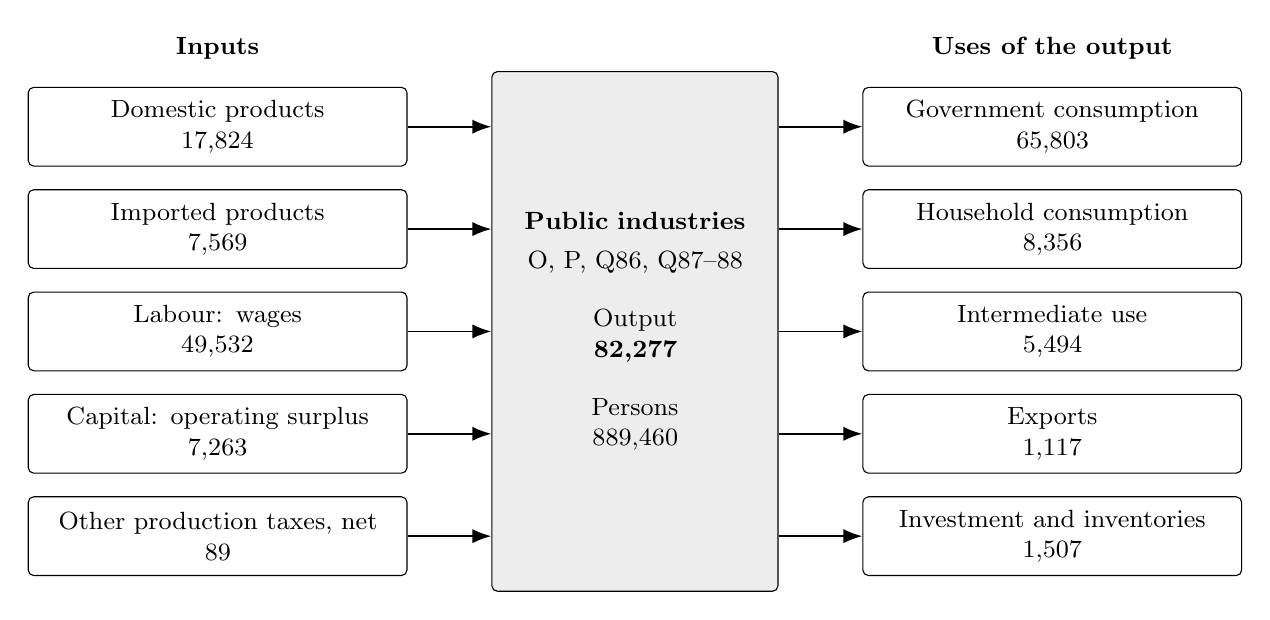
\begin{tikzpicture}[
  font=\small,
  box/.style={draw, rounded corners=2pt, align=center, inner sep=3pt, minimum height=10mm, text width=46mm},
  flow/.style={-{Latex[length=2.4mm]}, line width=0.6pt},
]
\node[draw, rounded corners=2pt, align=center, fill=black!7, text width=34mm, minimum height=66mm] (ind) at (0,0)
  {\textbf{Public industries}\\[3pt] O, P, Q86, Q87--88\\[10pt] Output\\ \textbf{82,277}\\[10pt] Persons\\ 889,460};
\node[font=\small\bfseries] at (-5.3,3.6) {Inputs};
\node[font=\small\bfseries] at (5.3,3.6) {Uses of the output};
\node[box] (i1) at (-5.3, 2.6) {Domestic products\\ 17,824};
\node[box] (i2) at (-5.3, 1.3) {Imported products\\ 7,569};
\node[box] (i3) at (-5.3, 0.0) {Labour: wages\\ 49,532};
\node[box] (i4) at (-5.3,-1.3) {Capital: operating surplus\\ 7,263};
\node[box] (i5) at (-5.3,-2.6) {Other production taxes, net\\ 89};
\node[box] (u1) at (5.3, 2.6) {Government consumption\\ 65,803};
\node[box] (u2) at (5.3, 1.3) {Household consumption\\ 8,356};
\node[box] (u3) at (5.3, 0.0) {Intermediate use\\ 5,494};
\node[box] (u4) at (5.3,-1.3) {Exports\\ 1,117};
\node[box] (u5) at (5.3,-2.6) {Investment and inventories\\ 1,507};
\foreach \n in {i1,i2,i3,i4,i5} \draw[flow] (\n.east) -- (\n.east -| ind.west);
\foreach \n in {u1,u2,u3,u4,u5} \draw[flow] (\n.west -| ind.east) -- (\n.west);
\end{tikzpicture}
\caption{Flows through the public industries, 2019. EUR million. Products are at purchaser prices on the input side and at basic prices on the output side. Of the intermediate use, the public industries take 3,016 themselves.}
\label{fig:flows}
\end{figure}

\paragraph{Products.}
The four industries buy products for 25,393 at purchaser prices. Domestic products are 17,824 and imports are 7,569.
The import share is 30 per cent. It is 39 per cent for all industries.
At basic prices the products are 21,666. Net product taxes are the other 3,727.
The model has no separate VAT rate yet, so VAT is in this item.

Table~\ref{tab:inputs} splits the purchases by product group.
The largest single products are IT services (J62--63, 2,555), pharmaceuticals (C21, 2,538), public administration services (O, 2,092), security, building, and office services (N80--82, 1,704), and real estate services (L, 1,458).
Health buys 1,981 of the pharmaceuticals. Imports are 96 per cent of the pharmaceuticals that the four industries buy.
The public industries also buy from each other: products O, P, and Q are 3,127 of their inputs.

\begin{table}[!htbp]
\centering
\small
\caption{Intermediate inputs of the public industries by product group, 2019. Purchaser prices, EUR million}
\label{tab:inputs}
\begin{tabular}{@{}lrrrrrr@{}}
\toprule
Product group (NACE section) & O & P & Q86 & Q87--88 & Sum & Of which imports \\
\midrule
Pharmaceuticals (C21) & 142 & 105 & 1,981 & 310 & 2,538 & 2,431 \\
Other manufactured goods (C) & 1,462 & 432 & 1,142 & 1,004 & 4,040 & 2,664 \\
Energy, water, and waste (D, E) & 237 & 491 & 423 & 465 & 1,615 & 65 \\
Construction (F) & 481 & 96 & 192 & 173 & 942 & 14 \\
Trade, transport, hotels (G, H, I) & 787 & 529 & 228 & 683 & 2,227 & 354 \\
Information and communication (J) & 1,549 & 1,146 & 523 & 180 & 3,398 & 949 \\
Finance and real estate (K, L) & 1,087 & 316 & 239 & 232 & 1,874 & 15 \\
Professional services and research (M) & 1,006 & 578 & 354 & 192 & 2,130 & 716 \\
Support services (N) & 751 & 637 & 708 & 579 & 2,674 & 209 \\
Public products (O, P, Q) & 935 & 747 & 828 & 616 & 3,127 & 88 \\
Other (A, B, R, S, T) & 53 & 164 & 159 & 450 & 826 & 64 \\
\midrule
Total & 8,490 & 5,241 & 6,778 & 4,884 & 25,393 & 7,569 \\
\quad of which net product taxes & 1,228 & 741 & 1,117 & 641 & 3,727 & \\
\bottomrule
\end{tabular}
\end{table}

\paragraph{Labour.}
Wages are 49,532, or 31 per cent of all wages in the economy. The four industries employ 889,460 persons.
Labour with tertiary education gets 33,333. This is 40 per cent of all tertiary wages.

\paragraph{Capital.}
The capital stock is 153,156 at the end of 2019. Structures are 103,330. Equipment, which includes intellectual property, is 49,826.
Fixed investment is 9,384, or 14 per cent of all fixed investment. Structures are 4,482 and equipment is 4,902.

The product accounts have one investment column for the whole economy. The model splits each capital type over products with fixed shares.
It does not record which products an industry invests in.
With the product mix of each capital type, the investment of the four industries is 4,097 of construction (F), 1,315 of research (M72), 766 of machinery (C28), 693 of motor vehicles (C29), 587 of IT services (J62--63), 525 of electronics (C26), and 1,401 of other products.

\section{Flows out of the public industries}

\subsection{Products made}

Each industry makes mainly the product with its own code. These four flows are 78,657, or 96 per cent of the output.
The other output is research services (M72, 2,560, of which 2,111 from education), public administration services from the other three industries (631), and other services (428).

Other industries make little of the four products. They make 383 of product O and 17 of product Q86.
Imports of the four products are 673.

\subsection{Uses}

The model does not record which industry supplies which user.
A product has one domestic basic price, and each industry makes a fixed share of the domestic supply.
Table~\ref{tab:uses} therefore applies the use pattern of each product to the output of each industry.

\begin{table}[!htbp]
\centering
\small
\caption{Uses of the output of the public industries, 2019. Basic prices, EUR million}
\label{tab:uses}
\setlength{\tabcolsep}{4pt}
\begin{tabular}{@{}lrrrrrrr@{}}
\toprule
 & \multicolumn{2}{c}{Intermediate use} & \multicolumn{4}{c}{Final use} & \\
\cmidrule(lr){2-3}\cmidrule(lr){4-7}
Industry & Public & Other & Government & Household & Exports & Investment & Output \\
 & industries & industries & consumption & consumption & & and inventories & \\
\midrule
O & 1,951 & 1,335 & 17,864 & 188 & 190 & 162 & 21,689 \\
P & 395 & 749 & 15,369 & 3,101 & 731 & 1,185 & 21,529 \\
Q86 & 658 & 356 & 16,880 & 2,139 & 114 & 145 & 20,291 \\
Q87--88 & 12 & 39 & 15,690 & 2,929 & 83 & 15 & 18,768 \\
\midrule
Four industries & 3,016 & 2,478 & 65,803 & 8,356 & 1,117 & 1,507 & 82,277 \\
Per cent & 3.7 & 3.0 & 80.0 & 10.2 & 1.4 & 1.8 & 100.0 \\
\bottomrule
\end{tabular}
\end{table}

Government consumption takes 80 per cent of the output. Households buy 10 per cent.
The exports and the investment of education come from its research output.

\subsection{Government consumption}

Government consumption is a column in the product accounts, as household consumption is. It is not the output of an industry or of a sector.
For each product, the value is a fixed share of nominal GDP:
\begin{equation}
p^G_{p,t}\, G_{p,t} = \mu^G_{p,t}\, V^{\GDP}_t .
\label{eq:g}
\end{equation}
The share $\mu^G_{p,t}$ is \code{rG2GDP_p}. The calibration sets it from the data of 2019, and it is constant from then.
The shares add to 24.3 per cent of GDP.
When the price of a public product rises more than nominal GDP, the quantity falls. The value share stays the same.

Table~\ref{tab:g} shows the column. Government consumption has 31 products.
The four public products are 88 per cent. The other 12 per cent are products of other industries.
Imports are 1,188 of the total, of which pharmaceuticals are 792.

\begin{table}[!htbp]
\centering
\small
\caption{Government consumption by product, 2019. Purchaser prices, EUR million}
\label{tab:g}
\begin{tabular}{@{}llrr@{}}
\toprule
Product & & Value & Per cent \\
\midrule
O & Public administration and defence & 18,709 & 25.0 \\
Q86 & Human health & 16,822 & 22.5 \\
Q87--88 & Residential care and social work & 15,627 & 20.9 \\
P & Education & 14,969 & 20.0 \\
\midrule
 & Four public products & 66,128 & 88.3 \\
\midrule
N78 & Employment activities & 1,412 & 1.9 \\
R90--92 & Arts, culture, and gambling & 1,246 & 1.7 \\
S94 & Membership organisations & 917 & 1.2 \\
F & Construction & 864 & 1.2 \\
C21 & Pharmaceuticals & 831 & 1.1 \\
H52 & Warehousing and transport support & 603 & 0.8 \\
 & 21 other products & 2,899 & 3.9 \\
\midrule
 & Government consumption, $V^G$ & 74,900 & 100.0 \\
\bottomrule
\end{tabular}
\end{table}

A change in government consumption goes through the model in this order.
Equation (\ref{eq:g}) sets the demand for each product. The demand goes to domestic supply and imports.
Domestic supply goes to the industries that make the product. Each industry then buys labour, capital, and products for its output.
Its price follows its marginal cost, and the price goes back into the purchaser price $p^G_{p,t}$.

\section{From the public industries to the government sector}
\label{sec:link}

\subsection{The share matrix}

The module \code{IndustrySectors} links industries to sectors with one matrix, $r_{s,i,t}$.
It is the share of industry $i$ that sector $s$ owns. The shares of the four domestic sectors add to one for each industry.
The shares are data. They are constant after 2019.

A sector gets the same share of all accounts of an industry:
\begin{align}
V^X_{s,t} &= \sum_i r_{s,i,t}\, V^X_{i,t}, \qquad X \in \{Y, M, W, \mathit{nt}, \mathit{sub}\}, \label{eq:share} \\
V^{\mathit{tax}}_{s,t} &= V^{\mathit{nt}}_{s,t} + V^{\mathit{sub}}_{s,t}, \\
V^B_{s,t} &= V^Y_{s,t} - V^M_{s,t} - V^W_{s,t} - V^{\mathit{nt}}_{s,t} . \label{eq:surplus}
\end{align}
The same shares give the persons, the capital stock, the consumption of fixed capital, and the fixed investment of each sector.
Gross capital formation adds a share of total inventory investment, $V^{\mathit{INV}}_t$:
\begin{equation}
V^I_{s,t} = \sum_i \sum_k r_{s,i,t}\, V^I_{k,i,t} + u_{s,t}\, V^{\mathit{INV}}_t .
\label{eq:investment}
\end{equation}
Here $k$ is the capital type and $u_{s,t}$ is \code{uINV_s}.

Figure~\ref{fig:link} and Table~\ref{tab:gov} show the result for the government sector.
Its output is 81,156. The four public industries give 59,602 of this, or 73 per cent.
The other 21,554 comes from 56 other industries.

\begin{figure}[!htbp]
\centering
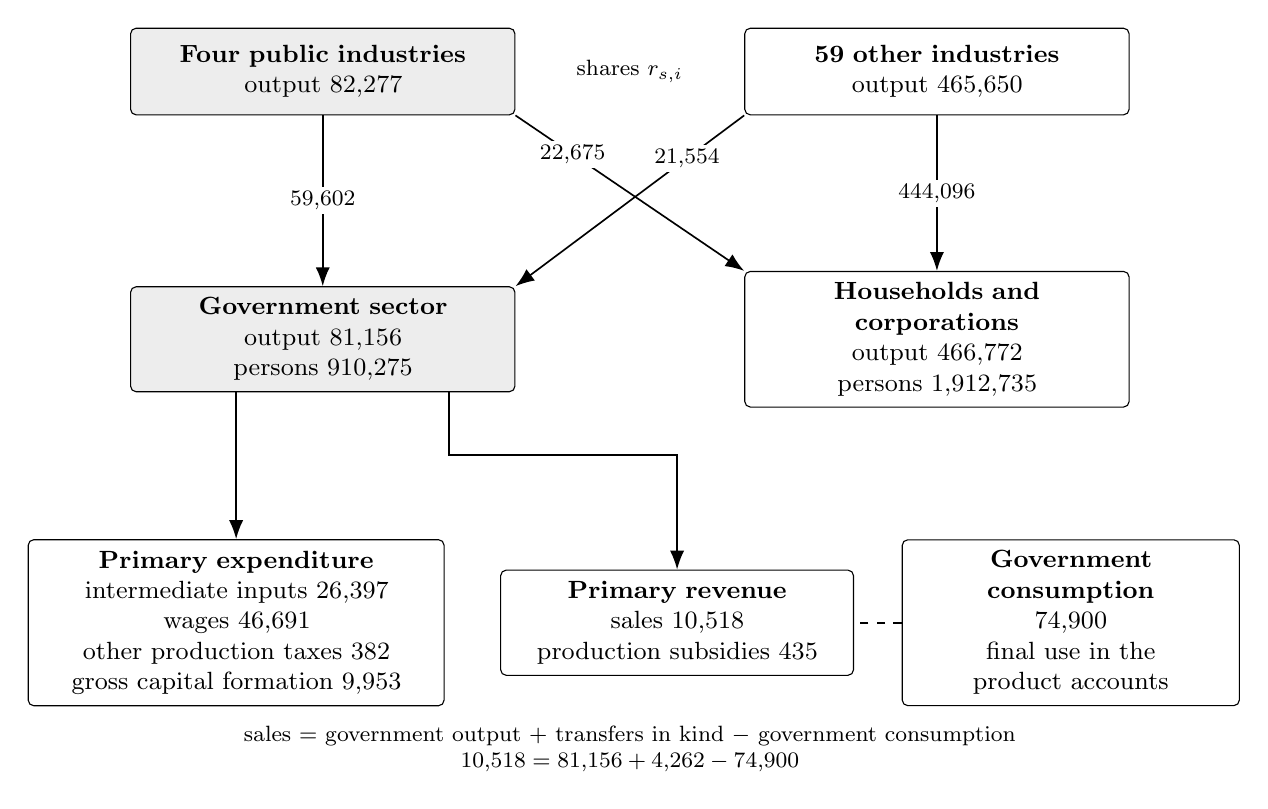
\begin{tikzpicture}[
  font=\small,
  box/.style={draw, rounded corners=2pt, align=center, inner sep=4pt, minimum height=11mm, text width=46mm},
  flow/.style={-{Latex[length=2.4mm]}, line width=0.6pt},
  lab/.style={font=\footnotesize, fill=white, inner sep=1.5pt},
]
\node[box, fill=black!7] (pub) at (-3.9,0) {\textbf{Four public industries}\\ output 82,277};
\node[box] (oth) at (3.9,0) {\textbf{59 other industries}\\ output 465,650};
\node[box, fill=black!7] (gov) at (-3.9,-3.4) {\textbf{Government sector}\\ output 81,156\\ persons 910,275};
\node[box] (prv) at (3.9,-3.4) {\textbf{Households and corporations}\\ output 466,772\\ persons 1,912,735};
\draw[flow] (pub.south) -- node[lab, pos=0.5] {59,602} (gov.north);
\draw[flow] (oth.south) -- node[lab, pos=0.5] {444,096} (prv.north);
\draw[flow] (pub.south east) -- node[lab, pos=0.25] {22,675} (prv.north west);
\draw[flow] (oth.south west) -- node[lab, pos=0.25] {21,554} (gov.north east);
\node[font=\footnotesize, align=center] at (0,0) {shares $r_{s,i}$};
\node[box, text width=50mm] (exp) at (-5.0,-7.0) {\textbf{Primary expenditure}\\ intermediate inputs 26,397\\ wages 46,691\\ other production taxes 382\\ gross capital formation 9,953};
\node[box, text width=42mm] (rev) at (0.6,-7.0) {\textbf{Primary revenue}\\ sales 10,518\\ production subsidies 435};
\node[box, text width=40mm] (g) at (5.6,-7.0) {\textbf{Government consumption}\\ 74,900\\ final use in the product accounts};
\coordinate (ga) at ([xshift=-11mm]gov.south);
\draw[flow] (ga) -- (ga |- exp.north);
\coordinate (gb) at ([xshift=16mm]gov.south);
\draw[flow] (gb) -- ++(0,-0.8) -| (rev.north);
\draw[dashed, line width=0.6pt] (g.west) -- (rev.east);
\node[font=\footnotesize, align=center] at (0,-8.6) {sales $=$ government output $+$ transfers in kind $-$ government consumption\\ $10{,}518 = 81{,}156 + 4{,}262 - 74{,}900$};
\end{tikzpicture}
\caption{From industries to the government budget, 2019. EUR million. The arrows from the industries show output. The same shares apply to inputs, wages, capital, and persons. The dashed line is identity (\ref{eq:sales}).}
\label{fig:link}
\end{figure}

\begin{table}[!htbp]
\centering
\small
\caption{The government sector by industry, 2019. EUR million}
\label{tab:gov}
\begin{tabular}{@{}lrrrrrrr@{}}
\toprule
 & & & \multicolumn{5}{c}{Government part of} \\
\cmidrule(l){4-8}
Industry & Share & Output & Output & Intermediate & Wages & Operating & Persons \\
 & $r_{\gov,i}$ & & & inputs & & surplus & \\
\midrule
P Education & 0.987 & 21,529 & 21,259 & 5,175 & 13,264 & 2,829 & 223,730 \\
Q86 Health & 0.916 & 20,291 & 18,591 & 6,210 & 10,937 & 1,301 & 187,794 \\
Q87--88 Social work & 0.983 & 18,768 & 18,446 & 4,801 & 13,300 & 464 & 294,533 \\
O Public administration & 0.060 & 21,689 & 1,307 & 511 & 640 & 151 & 9,533 \\
\midrule
Four public industries & 0.724 & 82,277 & 59,602 & 16,697 & 38,142 & 4,745 & 715,590 \\
\midrule
N78 Employment activities & 0.905 & 3,897 & 3,526 & 1,000 & 2,424 & 115 & 48,884 \\
G47 Retail trade & 0.223 & 14,318 & 3,189 & 1,238 & 1,597 & 358 & 52,245 \\
57 other industries & 0.033 & 447,436 & 14,838 & 7,462 & 4,528 & 2,903 & 93,556 \\
\midrule
Government sector & 0.148 & 547,927 & 81,156 & 26,397 & 46,691 & 8,121 & 910,275 \\
Source data & & & & 26,397 & 46,691 & 8,121 & \\
\bottomrule
\end{tabular}
\end{table}

\FloatBarrier
\subsection{Where the shares come from}

\code{IndustrySectorsData.jl} builds the shares. For the government it has three steps.
\begin{enumerate}
\item The starting value is a share of one for the industries in sections O, P, and Q, zero for finance (K), and a small share for all other industries.
\item An optimisation then fits the shares to four numbers in the source data for the government sector: intermediate consumption (P.2), employee compensation (D.1), other production taxes less subsidies (D.29 less D.39), and gross operating surplus.
\item The distance to the starting value enters the objective with a weight of $10^{-8}$.
\end{enumerate}
The last two rows of Table~\ref{tab:gov} show that the totals match. The four targets do not set the split over 60 industries.
Section~\ref{sec:shares} shows what the present split is and why.

\subsection{Government consumption and government output}

The product accounts give government consumption, $V^G_t$. The share matrix gives government output, $V^Y_{\gov,t}$.
No product flow links the two. One identity in \code{GovernmentRevenue} does:
\begin{equation}
V^{\mathit{sales}}_t = V^Y_{\gov,t} + V^{\mathit{kind}}_t - V^G_t .
\label{eq:sales}
\end{equation}
This is the definition of government consumption in the national accounts, solved for sales.
Government consumption is the output of the government sector that it does not sell, plus the products that it buys from market producers for households.
In 2019 the identity is $81{,}156 + 4{,}262 - 74{,}900 = 10{,}518$. The data value of sales is 10,518.

In the model, sales are the residual. If government output rises and government consumption does not, sales revenue rises by the same amount.
Social transfers in kind are a fixed share of government consumption, 5.7 per cent.

\subsection{The budget}

Table~\ref{tab:budget} shows the budget in 2019. The last column shows where each item comes from.
Five items come from the public industries and the other industries through the share matrix.
Sales come from identity (\ref{eq:sales}).

\begin{table}[!tb]
\centering
\small
\caption{The government budget, 2019. EUR million}
\label{tab:budget}
\begin{tabular}{@{}lrl@{}}
\toprule
 & Value & Source in the model \\
\midrule
Taxes on production and imports & 48,833 & Product and production tax rates \\
Current taxes on income and wealth & 96,624 & Tax rates on income \\
Sales & 10,518 & Identity (\ref{eq:sales}) \\
Production subsidies received & 435 & \textbf{Industry accounts and shares} \\
Equity income & 1,202 & Payout rate on equity assets \\
Social contributions & 2,644 & Share of the transfer index \\
Other current transfers & 3,312 & Share of gross value added \\
Capital taxes & 1,148 & Rate on household financial assets \\
Capital transfers & $-330$ & Share of gross value added \\
\textbf{Primary revenue} & \textbf{164,387} & \\
\midrule
Intermediate inputs & 26,397 & \textbf{Industry accounts and shares} \\
Wages & 46,691 & \textbf{Industry accounts and shares} \\
Other production taxes paid & 382 & \textbf{Industry accounts and shares} \\
Gross capital formation & 9,953 & \textbf{Industry accounts and shares} (\ref{eq:investment}) \\
Subsidies on products & 1,858 & Subsidy rates, less the part from abroad \\
Subsidies on production & 3,232 & Subsidies by industry, less the part from abroad \\
Social benefits in cash & 48,996 & Share of the transfer index \\
Social transfers in kind & 4,262 & Share of government consumption \\
Other current transfers & 9,361 & Share of gross value added \\
Capital transfers & 685 & Share of gross value added \\
Non-produced assets & $-419$ & Share of gross value added \\
\textbf{Primary expenditure} & \textbf{151,397} & \\
\midrule
\textbf{Primary balance} & \textbf{12,990} & \\
Interest received & 2,506 & ECB rate plus a fixed gap, on debt assets \\
Interest paid & 2,281 & ECB rate plus a fixed gap, on debt liabilities \\
\textbf{Balance} & \textbf{13,215} & 4.3 per cent of GDP \\
\bottomrule
\end{tabular}
\end{table}

The transfer index is the household wage sum two years before.
Government consumption is not a row in the table. The budget follows the government accounts: it has the costs of production on the expenditure side and the sales on the revenue side.

\subsection{The balance in net terms}

Put identity (\ref{eq:sales}) into the budget, and use (\ref{eq:surplus}) for the government sector.
Output, intermediate inputs, wages, and production taxes and subsidies of the government sector then leave the balance. Only the operating surplus is left:
\begin{equation}
\mathit{PB}_t = T_t + R_t + V^B_{\gov,t} - V^G_t - V^I_{\gov,t} - S_t - H_t - E_t .
\label{eq:net}
\end{equation}
$\mathit{PB}_t$ is the primary balance. $T_t$ is taxes. $R_t$ is the other revenue without sales and subsidies received.
$S_t$ is subsidies paid, $H_t$ is social benefits in cash, and $E_t$ is other transfers and non-produced assets.
In 2019 the terms are
\[
145{,}457 + 7{,}976 + 8{,}121 - 74{,}900 - 9{,}953 - 5{,}090 - 48{,}996 - 9{,}626 = 12{,}990 .
\]

Equation (\ref{eq:net}) shows what the link between the public industries and the budget is.
\begin{itemize}
\item \textbf{The net expense is government consumption.} The government pays the purchaser price for the products in column G. It does not matter for the balance who makes them.
\item \textbf{Wages in the public industries do not enter directly.} A higher wage raises the price of the public products. Equation (\ref{eq:g}) holds the value of government consumption at a fixed share of GDP, so the quantity falls.
\item \textbf{The shares matter through two terms only.} A higher government share of an industry moves operating surplus and investment of that industry to the government. Output, inputs, and wages of the government sector change, but they cancel.
\end{itemize}

The balance goes to the financial accounts. The government does not trade equity or debt assets, and its debt liabilities take the whole balance.
The model has no fiscal rule. The note \code{mirror_closure.tex} describes the result for the debt.

\section{The present shares}
\label{sec:shares}

\subsection{Public administration}

The government share of public administration is 0.060. The starting value in the data build is one.
Non-financial corporations get 0.920 of the industry, and households get 0.020.
The government gets large shares of two industries outside sections O, P, and Q: employment activities (0.905) and households as employers (0.836).

A test for this note ran the function \code{build_industry_sector_shares} again with the same data and other weights on the starting value.
Table~\ref{tab:test} shows the result. The first row is the code now, and it gives the shares in the data file.
With a weight of $10^{-4}$ the four shares are from 0.90 to 0.93, and the government sector still matches the government accounts.
The four public industries then give 76,130 of the government output, or 94 per cent.
The weight $10^{-8}$ is too small to hold the shares near the starting value.

\begin{table}[!htbp]
\centering
\small
\caption{Government shares for different weights on the starting value, 2019}
\label{tab:test}
\begin{tabular}{@{}lrrrrrrrr@{}}
\toprule
 & \multicolumn{5}{c}{Government share} & \multicolumn{3}{c}{Government sector, EUR million} \\
\cmidrule(lr){2-6}\cmidrule(l){7-9}
Weight & O & P & Q86 & Q87--88 & N78 & Output from the & Intermediate & Wages \\
 & & & & & & four industries & inputs & \\
\midrule
$10^{-8}$ (code now) & 0.060 & 0.987 & 0.916 & 0.983 & 0.905 & 59,602 & 26,397 & 46,691 \\
$10^{-6}$ & 0.743 & 0.987 & 0.826 & 0.985 & 0.075 & 72,625 & 26,397 & 46,691 \\
$10^{-4}$ & 0.933 & 0.932 & 0.904 & 0.933 & 0.004 & 76,130 & 26,397 & 46,691 \\
$10^{-2}$ & 0.939 & 0.935 & 0.909 & 0.936 & 0.000 & 76,513 & 26,365 & 46,724 \\
\midrule
Source data & & & & & & & 26,397 & 46,691 \\
\bottomrule
\end{tabular}
\end{table}

The test changed no file in the repository. The model was not calibrated with the test shares.

The present shares have these effects in the model.
\begin{itemize}
\item \textbf{Levels.} The government totals for intermediate inputs, wages, and operating surplus match the government accounts. The budget in 2019 is not affected.
\item \textbf{Responses.} The government sector gets 27 per cent of its output from 56 industries outside the public industries. A shock to private demand for their products moves government output, wages, persons, and sales revenue. A shock to public administration moves them very little.
\item \textbf{Persons.} Government employment is 910,275 persons. Only 9,533 of the 158,240 persons in public administration are in it. It has 48,884 of the 54,020 persons in employment activities.
\item \textbf{Capital cost.} The marginal corporation tax rate of an industry is the tax rate times the corporate share of the industry. It is 0.327 in public administration and below 0.03 in the other three public industries. The capital user cost of public administration therefore includes corporation tax.
\item \textbf{Corporation tax base.} Non-financial corporations get 2,306 of the operating surplus of public administration (2,506). This amount is in their taxable income.
\item \textbf{Sales.} With the use pattern of each product, 49,422 of the government output of 81,156 goes to government consumption. Identity (\ref{eq:sales}) does not use this number. It takes sales as the residual, 10,518.
\end{itemize}

\subsection{Other differences between the shares and the source data}

\begin{itemize}
\item \textbf{Gross capital formation.} The sector accounts give 9,953 for the government. The shares give fixed investment of 8,068. The calibration puts the difference of 1,885 in the inventory share $u_{\gov}$, which becomes 1.24. Total inventory investment is 1,521 in 2019 and halves each year. The inventory part of government capital formation is 932 in 2020 and close to zero in 2030. Government capital formation is 8,244 in 2020 and 7,473 in 2030.
\item \textbf{Consumption of fixed capital.} The government accounts give 8,121. The shares give 6,377. The model keeps the data value in 2019 and uses the share value from 2020. No other equation uses this variable.
\item \textbf{Production subsidies received.} The sector accounts give 435. The shares give 358. The model uses the share value from 2020.
\end{itemize}

\section{Limits of this note}

\begin{itemize}
\item The numbers are from the baseline file of 12 November 2026 and the data files in \code{model_julia/data}. The model was not solved for this note.
\item All tables are for 2019. The baseline is close to constant in adjusted values, so the shares of GDP change little. Government consumption is 24.3 per cent of GDP in all years.
\item Table~\ref{tab:uses}, the investment by product in Section~\ref{sec:in}, and the last point on sales in Section~\ref{sec:shares} are calculations of this note. They use the fixed shares of the model. They are not model variables.
\item The name public industries is a choice of this note. The model does not use it.
\item The test in Table~\ref{tab:test} shows that the weight explains the share of public administration. It does not show which weight is best.
\item The scripts that made the tables are not in the repository.
\end{itemize}

\end{document}
